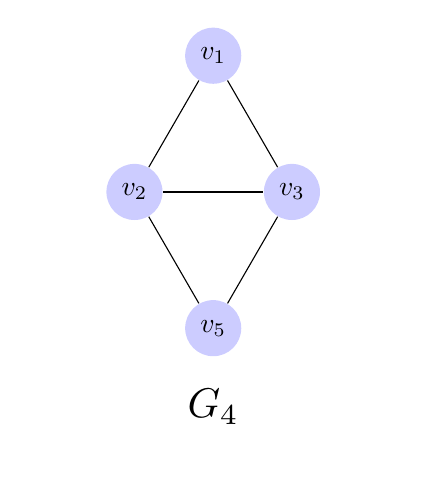
\begin{tikzpicture}
  [scale=1,auto=left,every node/.style={circle,fill=blue!20}]
  % Posiciones simétricas en forma de triángulo equilátero
  \node (n1) at (2,3.46) {$v_1$};
  \node (n2) at (1,1.73) {$v_2$};
  \node (n3) at (3,1.73) {$v_3$};
  \node (n4) at (0,0)   [opacity=0] {$v_4$};
  \node (n5) at (2,0)    {$v_5$};
  \node (n6) at (4,0)   [opacity=0] {$v_6$};

  % Aristas del grafo base (malla triangular)
  \foreach \from/\to in {n1/n2, n1/n3, n2/n3, n2/n5, n3/n5}
    \draw (\from) -- (\to);

   \node[draw=none, fill=none, scale=1.5] at (2,-1) {$G_4$};
\end{tikzpicture}
